%!TEX root = Main.tex
% Implementation: words
\chapter{Implementation} % (fold)
\label{cha:system_design}

\section{System Overview} % (fold)
\label{sec:system_overview}
	The hardware related goals outlined in Chapters 1 and 2 can be summarised as:
	\begin{enumerate}
		\item Design a system in programmable logic that can efficiently evaluate Equation~\ref{eq:score_final}.
		\item Design a C program to pre-process speech data according to the required form described in Section~\ref{sec:the_hmm_based_model}.
	\end{enumerate}

	The overall system layout, shown in Figure~\ref{fig:hlsystem}, is comprised of two primary blocks -- the processor and the FPGA (on L'Imperatrice and La Papessa boards respectively).  The entire system is powered from a single supply connected to the L'Imperatrice battery connector; La Papessa is powered through a ribbon cable between the two boards.  This was done in order to minimise the amount of external circuitry needed, and to show that the two devices are able to work together fairly easily.

	From the list above, the first task is implemented on La Papessa, and the second on L'Imperatrice.  These two blocks will now be examined in greater detail.

	% How to display which tasks are accomplished by which parts?

	% TODO:
	% Diagram of the ribbon cable connections (ie which pins do what)

	\begin{figure}[tb]
		\begin{center}
			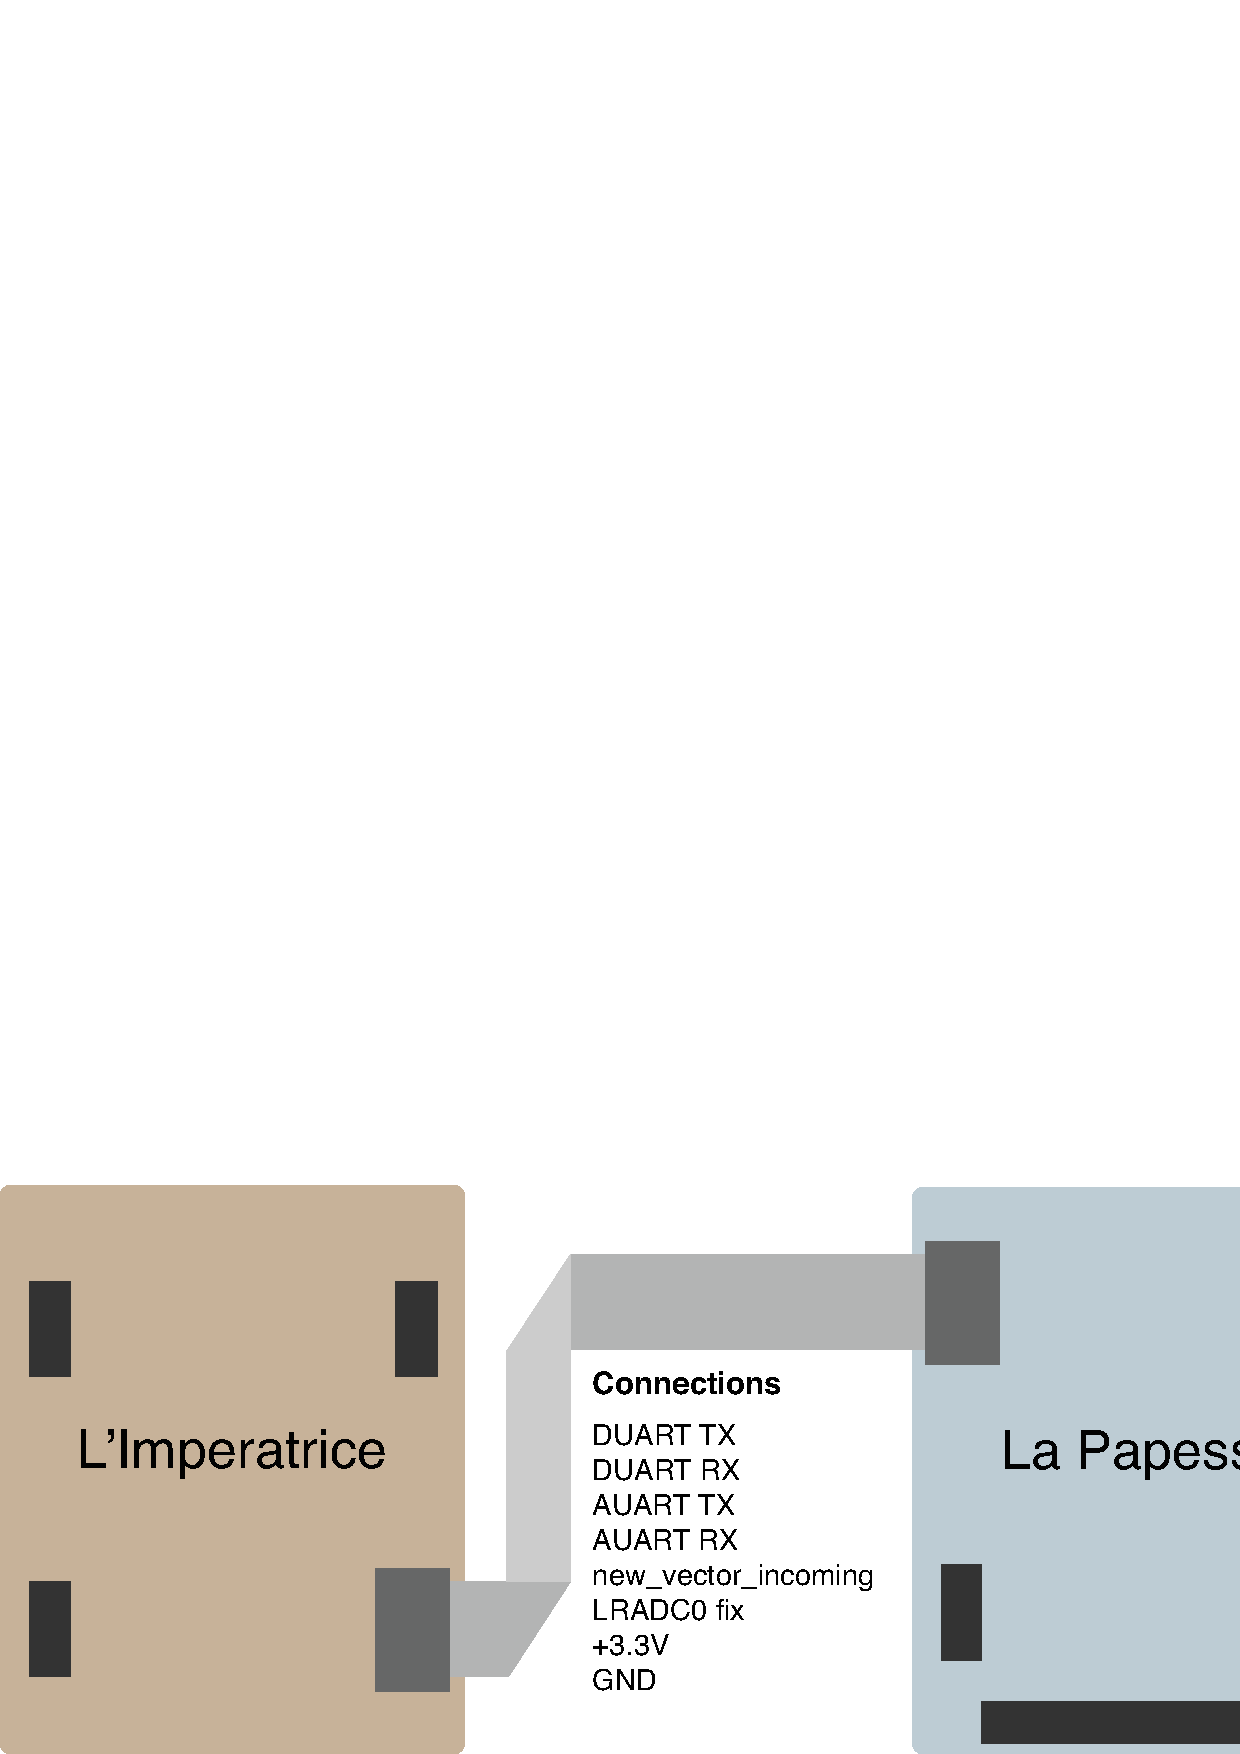
\includegraphics[width=\figwidth]{complete-system-overview.png}
		\end{center}
		\caption{Complete system overview}
		\label{fig:hlsystem}
	\end{figure}
% section system_overview (end)


\section{Number Format} % (fold)
\label{sec:number_format}
	% 16 bit numbers, scaling up and down
	% How were these chosen?
	Before beginning implementation of any part of the project, a number representation which would be appropriate for the FPGA had to be decided upon.  Firstly, it was recognised that using floating-point arithmetic on the FPGA would not be worth the effort, and therefore some form of fixed-point system was needed.  Further, the number magnitudes vary greatly between stages and parameters in the system.  In order to solve this problem, different scaling factors were used to bring most of the parameters to a similar magnitude.  

	The inputs and outputs of the Gaussian Distance Pipe, the module that performs the core calculation, are all signed 16-bit fixed point numbers, with varying scaling factors.  In particular, the $k$ parameter was generally larger than $x$, $mean$, and $omega$, and thus was scaled down.  The scaling factors were decided primarily by analysing the HMM models, to determine the largest and smallest numbers used.

	These decisions were influenced by Melnikoff \cite{melnikoff2003speech}, and the HTK, as they both use scaled 16-bit numbers to represent the parameters and scores.
% section number_format (end)


\section{La Papessa (The FPGA)} % (fold)
\label{sec:la_papessa_fpga}
	% The development environment used (Detailed documentation in Appendix)
	% GD Pipeline
	% SRAM
	% Controller
	% Normaliser pipeline
	% Communications

	The system on La Papessa performs these main tasks:
	\begin{itemize}
		\item Receives observation vectors from L'Imperatrice.
		\item Computes the score (Equation~\ref{eq:score_final}) of every senone in the model, with the given observation.
		\item Normalises the senone scores.
		\item Sends the scores back to L'Imperatrice.
	\end{itemize}

	\subsection{Top Level Module} % (fold)
	\label{sub:top_level_module}
		A simplified diagram of the top level module is given in Figure~\ref{fig:toplevel}, showing the main components of the system.  This module included the main controller logic, which essentially waited for a new observation vector, then cycled through the necessary operation states.  Figure~\ref{fig:topstatemachine} shows an ASM of this logic, and also outlines the main areas of the design that need explanation.

		The top level module is also responsible for handling access to the on-board SRAM chip, which several modules need to write or read from.  It essentially multiplexes the required signals, and leaves them floating (high impedance) when they are not needed.  The ``Debug signals'' shown in Figure~\ref{fig:toplevel} are a number of internal signals that are routed to output ports in order to facilitate hardware debugging.

		\begin{figure}[tb]
			\begin{center}
				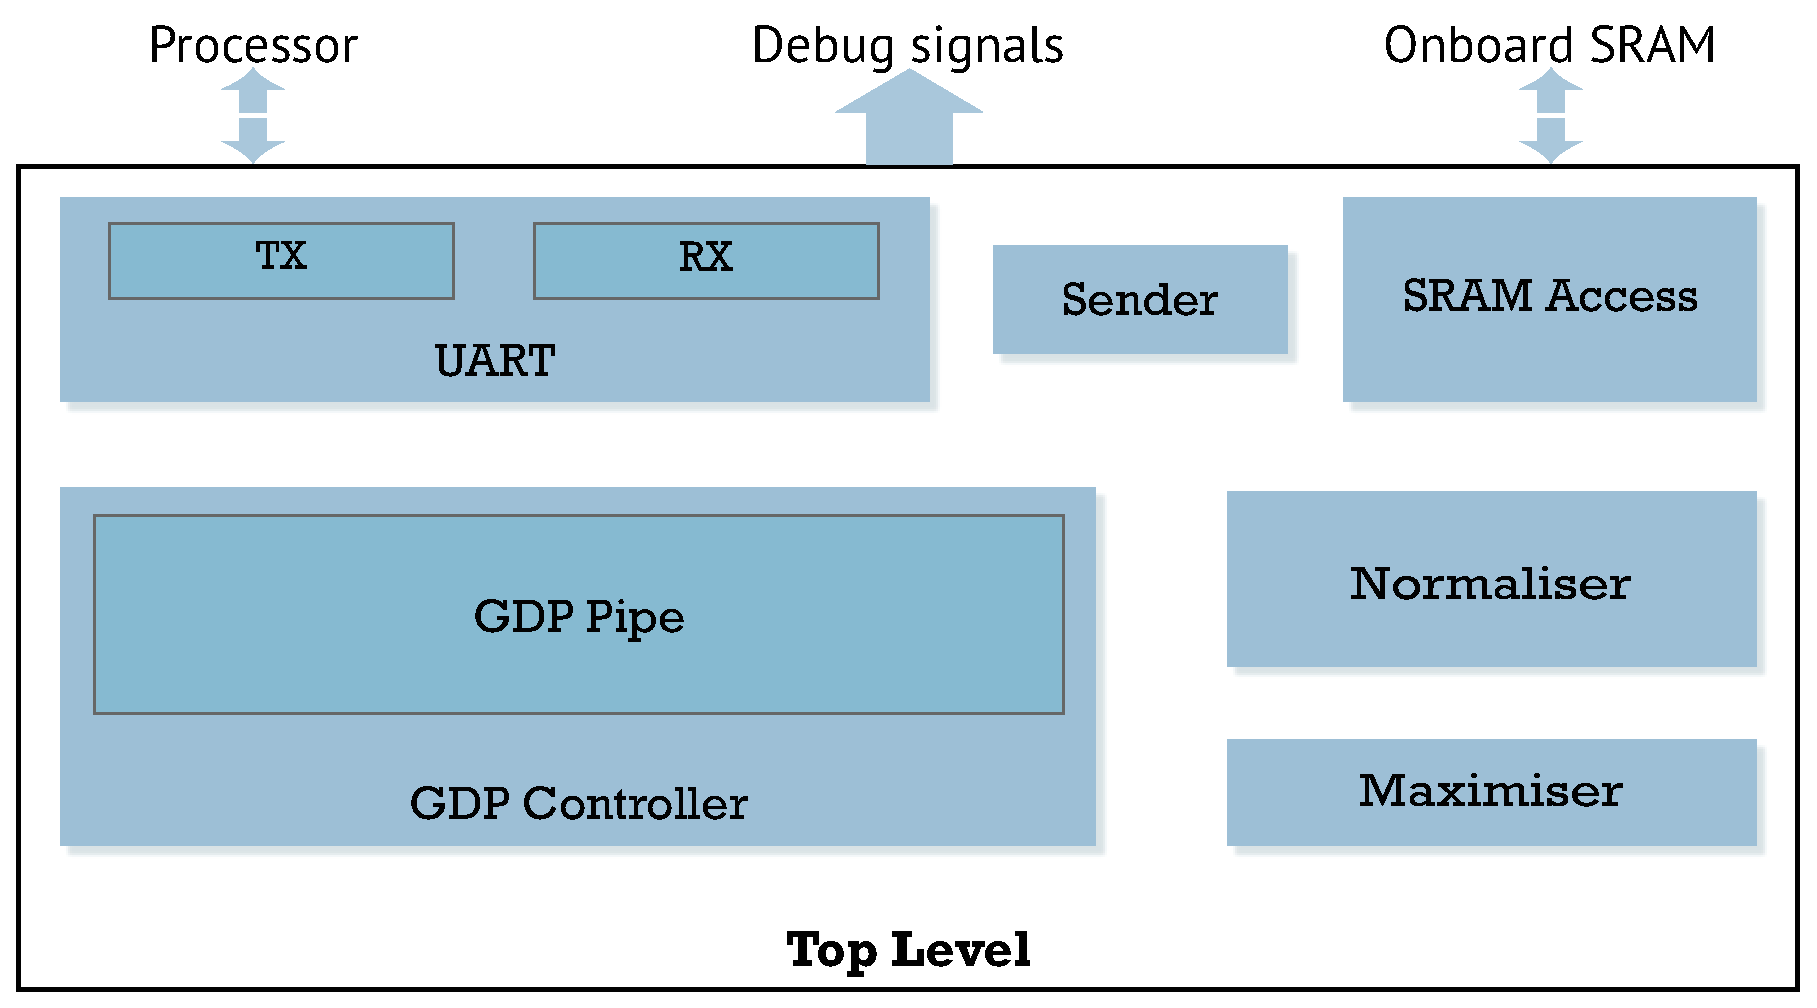
\includegraphics[width=\textwidth]{top_level}
			\end{center}
			\caption{Component diagram of the Top Level Module (Section~\ref{sub:top_level_module})}
			\label{fig:toplevel}
		\end{figure}

		\begin{figure}[tb]
			\begin{center}
				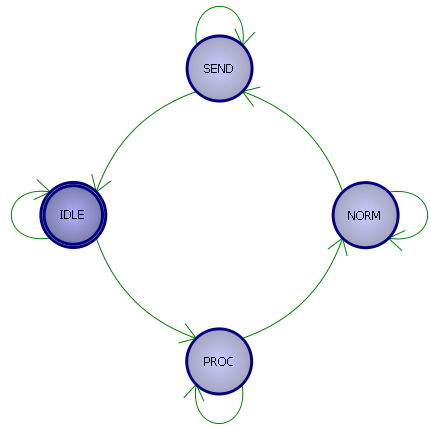
\includegraphics[width=0.6\textwidth]{TopLevel_asm}
			\end{center}
			\caption{ASM diagram of Top Level Module (Section~\ref{sub:top_level_module})}
			\label{fig:topstatemachine}
		\end{figure}
	% subsection top_level_module (end)

	\subsection{Gaussian Distance Pipeline} % (fold)
	\label{sub:gaussian_distance_pipeline}
		The Gaussian Distance Pipeline (GDP)\nomenclature{GDP}{Gaussian Distance Pipeline} is the core component of the system, and computes Equation~\ref{eq:score_final}.  It is a relatively simple 4-stage pipeline, with one stage for every step in the equation (subtract, square, scale, accumulate).  Although the gains from using a pipeline in this case are relatively small, it would be very useful if more complex models were used.  The Speech Silicon \cite{schuster2006speech} project had a substantially more complex GDP, as their senones have several Gaussian distributions that must be mixed to produce the final output distribution.  A block diagram of the GDP module is shown in Figure~\ref{fig:gdp_block}.  %TODO: describe the inputs etc...

		\begin{figure}[tb]
			\begin{center}
				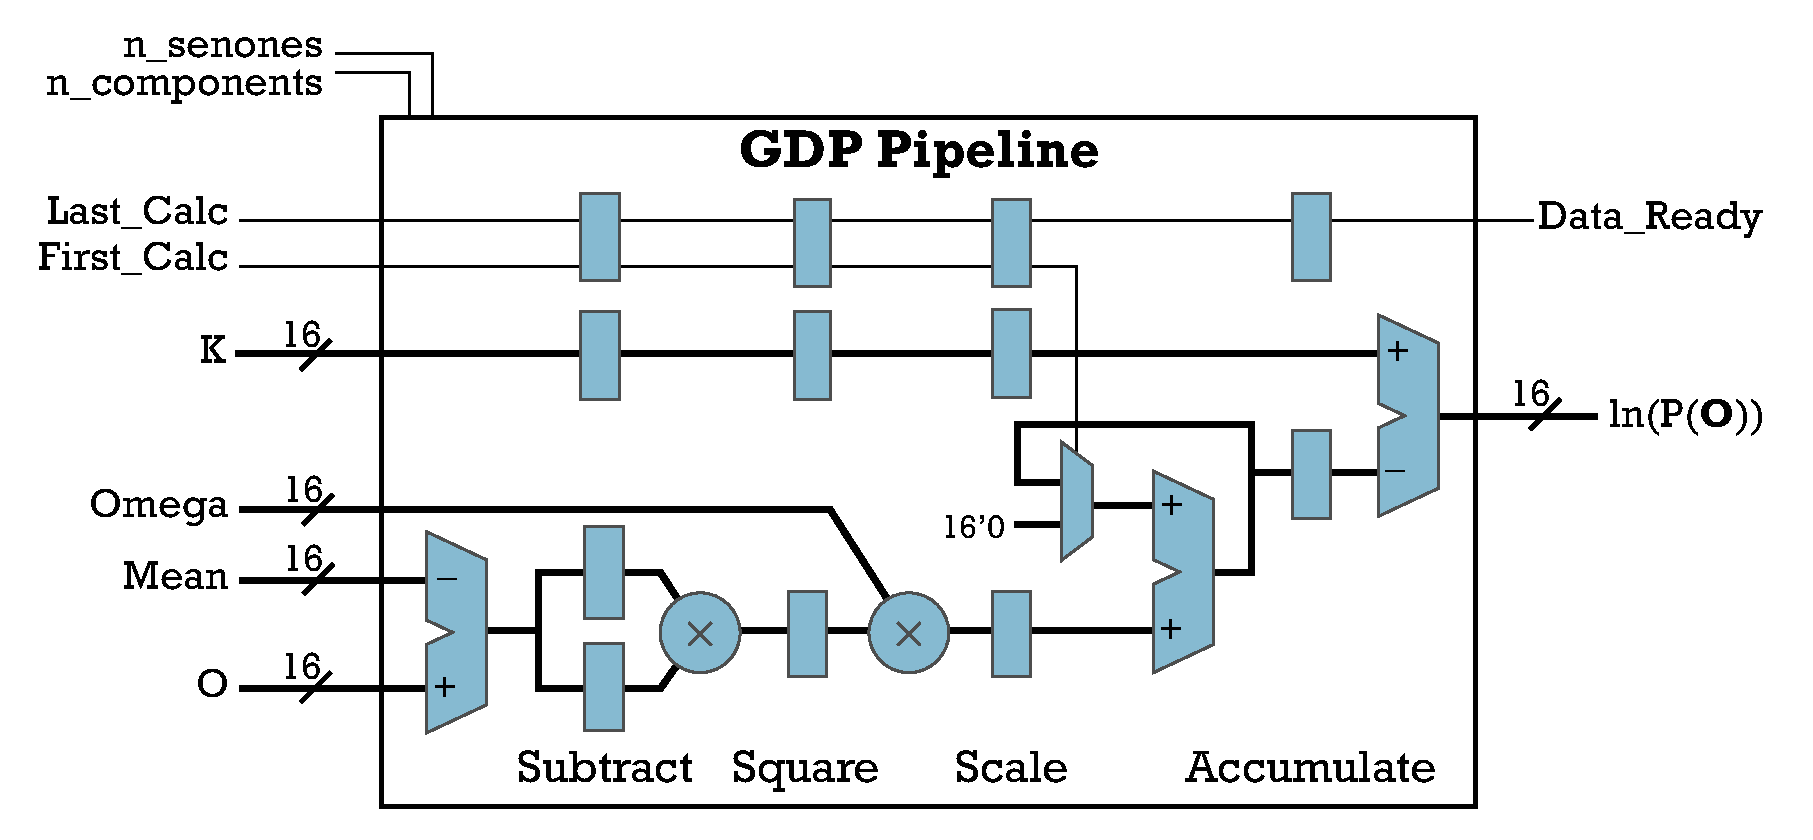
\includegraphics[width=\textwidth]{gdp_module_block}
			\end{center}
			\caption{Gaussian Distance Pipeline block diagram}
			\label{fig:gdp_block}
		\end{figure}

		In this module, `\texttt{n\_senones}' and `\texttt{n\_components}' are both parameter inputs, which determine the number of senones and the number of components per mean and variance in the model.  This allowed the design to be scaled down as size constraints became restrictive.

		The pipeline itself is a static object without much control logic, and thus requires a controller which sequentially uses it to score each senone in the model.  This controller is a simple state machine of only two states (\texttt{IDLE} and \texttt{LOAD\_GDP}), which begins feeding the pipe when a `\texttt{new\_vector\_available}' input flag is asserted.  This module is shown in Figure~\ref{fig:gdp_ctrl_block}.  A `\texttt{last\_senone}' output flag is asserted when the GDP produces the last senone score.  When the controller is in the \texttt{LOAD\_GDP} state, it essentially loops through the senones in the model, extracting their parameters and sending them to the GDP.  

		In order to facilitate the extraction and manipulation of senone parameters, a SystemVerilog structure was created, shown in Listing~\ref{lst:senonestr}. A SystemVerilog ROM module, connected to the controller, was populated with the senone parameters, stored in this structure.  Thus, when `\texttt{new\_vector\_available}' is asserted, the controller simply counts from 0 up to \texttt{n\_senones} (the number of senones in the model), and pulls the required parameters out of the ROM.

\begin{lstlisting}[style=customc, label=lst:senonestr, caption=Senone parameter data structure]
typedef struct packed {  /* num: typedef logic signed [15:0] num; */
  num k;
  num [n_components-1:0] omegas;
  num [n_components-1:0] means;
} senone_data;
\end{lstlisting}

		After asserting \texttt{new\_vector\_available}, and providing the relevant vector on the `\texttt{x}' input, the top level module will see  senone scores being sequentially produced, along with an index or ID which is unique to each senone.  The Top Level module is then responsible for storing the score in SRAM, and a ``Maximiser'' module registers the highest score seen.
		%TODO: show a multisim diagram of the normaliser??
		%TODO: where does it get its data from???
		\begin{figure}[tb]
			\begin{center}
				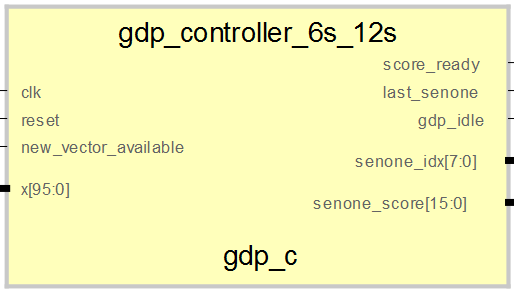
\includegraphics[width=\figwidth]{gdp_ctrl_block.png}
			\end{center}
			\caption{Gaussian Distance Pipe Controller block diagram}
			\label{fig:gdp_ctrl_block}
		\end{figure}
	% subsection gaussian_distance_pipeline (end)

	\subsection{Normalising Scores} % (fold)
	\label{sub:normaliser}
		The Speech Silicon architecture included a module which normalised the senones before they were used for decoding.  A very similar module is implemented here to perform the same normalisation.  The highest score is found while senones are being evaluated, and then this score is subtracted from all the final scores.  This causes the senone with the highest score to have a score of 0, which corresponds to a probability of 1 (the scores are log probabilities, see Section \ref{sub:senone_scoring}).
	% subsection normaliser (end)

	\subsection{SRAM} % (fold)
	\label{sub:onboard_sram}
		In order for the normaliser to access the senone scores, they must be stored somewhere as they are processed through the GDP.  One option would be to store them on the FPGA itself, where they would be accessible to all the modules.  However, this is impractical due to the potential size of an HMM model, and thus the large amount of RAM that would be required.  A better alternative would be to use external SRAM with low latency that is made accessible to whichever modules need it.

		Revision C of La Papessa board includes an on-board SRAM chip, which has an 8 bit data bus and 21 bit address bus, and was completely untested before this work.  In order to use it easily, a module was created primarily to interface the 8 bit data bus with the 16 bit number system used.  It's only operations are to write and read 16 bit values to the SRAM, and signal when it is ready or idle.  This is accomplished with the state machine shown in Figure~\ref{fig:sram_asm}.

		\begin{figure}[tb]
			\begin{center}
				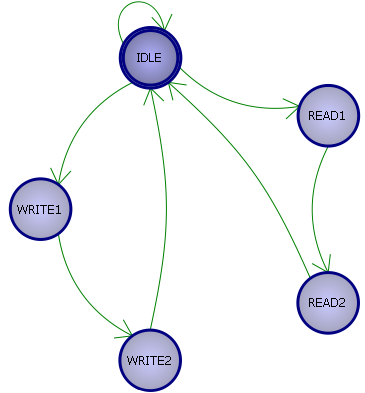
\includegraphics[width=0.6\textwidth]{SRAM_asm}
			\end{center}
			\caption{ASM of the SRAM access module (\ref{sub:onboard_sram})}
			\label{fig:sram_asm}
		\end{figure}
	% subsection onboard_sram (end)

	\subsection{Communications} % (fold)
	\label{sub:fpga_communications}
		The primary method of communication between the FPGA and processor is a standard UART bus, running at 115200 baud.  The communications module on the FPGA is essentially comprised of standard UART receive/transmit modules and a module that is wrapped around them to provide a higher level of data abstraction.  Because numbers are all 16 bits long in this system, and UART words are normally 8 bits, one of the wrapper purposes is to receive and transmit 16 bit numbers.  In addition, it is known beforehand that the FPGA should receive a certain number of bytes per observation vector.  This allows the UART module to wait until a 'packet' with that number of bytes has arrived, before signalling to the main controller that a new vector has arrived.  In this implementation, a buffer is simply filled up as new bytes arrive, and then is passed to the main controller when full.  However, it may happen that the UART module erroneously receives a byte, causing the buffer to be one byte fuller than it should be, and therefore causing the last byte of a new observation to be dropped.  In order to work around this, a `\texttt{new\_vector\_incoming}' flag is added, which will empty the buffer when asserted by the processor.  Another (possibly better way) of avoiding errors would be to automatically empty the buffer if new data is not received for a time-out period.  However, this is left as a possible future enhancement, as the \texttt{new\_vector\_incoming} flag is sufficient for now.

		The Baudticker module generates clock signals for the transmit and receive modules.  The transmit module requires a signal at approximately 115200Hz, but the receive module requires a signal at 8 times that frequency.  The receiver oversamples the input \texttt{rx} signal at this higher frequency, which enables it to detect and ignore signal glitches.  % TODO: finish this

		The Sender module is fairly simple in its operation -- it loops through all the senone scores stored in external SRAM and sends them over UART to the processor.
	% subsection fpga_communications (end)

% section la_papessa_fpga (end)


\section{L'Imperatrice (The processor)} % (fold)
\label{sec:l_imperatrice_processor}
	% GPIO
	% App UART
	% FFTW - compilation, LTIB, usage
	% LibMFCC
	% Various bits from HTK (liftering etc)
	% Makefile

	L'Imperatrice performs these main tasks:
	\begin{itemize}
		\item Read speech data from a WAV file.
		\item Pre-process -- pre-emphasise and window data, calculate FFT, calculate MFCCs, `Lifter' MFCCs.
		\item Convert MFCCs to the correct binary format.
		\item Send this observation vector to La Papessa.
		\item Receive and display scores.
	\end{itemize}

	% The most important task is the pre-processing -- Once this is done, it is a fairly simple matter to convert it to the correct 16-bit binary format, send the observation, and display the received scores.  

	\subsection{Pre-processing} % (fold)
	\label{sub:pre_processing}
		Instead of reading data in from a microphone, the system uses pre-recorded speech stored in WAV formatted audio files.  This method was chosen because it allows the pre-processing to be very easily tested, without worrying that the input data was changing.  In addition, it allowed the results to be compared with pre-processed data from other libraries, such as the HTK, in order to verify correct operation.

		The audio files were prepared specially, in a format that is simple to read and use.  The audio manipulation software `Audacity'\footnote{Audacity is available at \href{http://audacity.sourceforge.net/}{http://audacity.sourceforge.net/}, last checked April 2013.} was used to record and store speech as uncompressed (Microsoft) WAV files with unsigned 8-bit PCM encoding.  As Audacity does not support saving files with 8kHz sampling rates, the `sox'\footnote{SOX (Sound eXchange) is available at \href{http://sox.sourceforge.net/}{http://sox.sourceforge.net/}, last checked April 2013.} utility was used to downsample them from 48kHz to 8kHz.

		In pre-processing the data, an attempt was made to match the processes that the HTK used as closely as possible, thus making it easier to verify that the process works correctly.  Samples from the audio files are read in sequential blocks of between 80 and 200 samples, depending on the window size required.  These blocks are windowed with a Hamming window to remove discontinuities at the edges which could cause excess spectral noise.  The DFT is taken of this data, using the FFTW library, which had to be specially packaged and compiled for use in LTIB (See Appendix~\ref{apdx:compiling_fftw_for_ltib}).  Finally, the magnitude is taken, so that the spectral data is fully real and may be used to calculate Mel Frequency Cepstral Coefficients (MFCCs).  An external library (LibMFCC) was used for this purpose, due to its availability and the time constraints on the project.  The last operation, shown in Equation~\ref{eq:ceplifter}, is to perform Liftering\footnote{The name ``Liftering'' comes from the HTK book \cite{htkbook}} on each of the coefficients, where $L$ is a parameter.  This results in the cepstral coefficients having similar magnitudes \cite{htkbook}, which is particularly convenient when they must be represented with a 16-bit fixed-point number.
		\meq{ceplifter}{
			{c^{\prime}}_n
			= \left(1 + \frac{L}{2} sin \frac{\pi n}{L}\right) c_n
		}
	% subsection pre_processing (end)

	\subsection{GPIO and Application UART} % (fold)
	\label{sub:gpio_application_uart}
		In order to communicate with the FPGA, the processor required access to a serial port.  The ideal solution is the built-in Application UART port on the iMX23 chip, which only needs configuring.  In addition, access to GPIO from inside a C program was required to assert the \texttt{new\_vector\_incoming} signal.

		Both GPIO and Application UART must be enabled by selecting the relevant entry in the Kernel configuration menu at compile time (See Appendix~\ref{apdx:ltib_usage}).  Using the Application UART from a C program requires opening the serial port file (\texttt{/dev/ttySP1}, usually) and using the \texttt{termios.h} library to configure it correctly.  The options used to configure the serial port are shown in Listing~\ref{lst:serialconfig}.

\begin{lstlisting}[style=customc, label=lst:serialconfig, caption=Serial Port Configuration]
/* Set important serial port parameters: */
stty.c_cc[VMIN] = 0;                          // No blocking read
stty.c_cc[VTIME] = 1;                         // 0.1s: Max wait for data
stty.c_cflag = (stty.c_cflag & ~CSIZE) | CS8; // 8 bit chars
stty.c_iflag &= ~IGNBRK;                      // Ignore break commands
stty.c_lflag = 0;
stty.c_oflag = 0;
stty.c_iflag &= ~(IXON | IXOFF | IXANY);      // No flow ctrl
stty.c_cflag |= (CLOCAL | CREAD);             // enable receiver
stty.c_cflag &= ~(PARENB | PARODD);           // No parity
stty.c_cflag &= ~CSTOPB;                      // Send 1 stop bit
stty.c_cflag &= ~CRTSCTS;
\end{lstlisting}

		The GPIO is accessible in more than one way -- either through sysfs or via direct register access.  The kernel is configured to include the sysfs GPIO interface, which creates an entry under \texttt{/sys/class/gpio} that allows GPIO pins to be written and read as standard files.  Alternatively, the `Olinuxino' board project (which uses the same processor as L'Imperatrice) includes C code to directly write and read the GPIO registers as mapped memory\footnote{Accessible on the Olinuxino Github repository at \href{https://github.com/OLIMEX/OLINUXINO/}{https://github.com/OLIMEX/OLINUXINO/}}.  The project uses the second method, as it was straightforward to adapt the existing code for the purposes of the project.  In addition, direct memory access is far faster than the sysfs gpio interface; in tests, it was capable of switching frequencies up to 2MHz while the sysfs interface only managed about 200Hz.

	% subsection gpio_application_uart (end)

	% \subsection{Build process} % (fold)
	% \label{sub:build_process}
	% 	TODO??
	% % subsection build_process (end)

% section l_imperatrice (end)


\section{Support Software} % (fold)
\label{sec:support_software}
	A set of utilities were written in Common Lisp in order to facilitate and accelerate various parts of the project development.  Common Lisp was chosen due to its extreme power and flexibility, and because the IDE used, Emacs SLIME, is considered superior to any other.  In particular, these utilities helped with the following tasks (See Appendix~\ref{apdx:lisp_utils} for documentation):
	\begin{itemize}
		\item Parsing HMM definitions created by HTK, and extracting senone parameters
		\item SystemVerilog testbench generation
		\item Senone data file generation
		\item Verifying hardware functionality
		\item Number format conversion tasks
	\end{itemize}

	The HTK stores HMM definitions (along with transition matrices and senone definitions) in a human-readable plain-text Ascii file.  However, due to the very large model size, it was impractical to attempt to copy out parameters by hand.  For this reason, a parser was created that read an HMM definition file and stored the extracted data in a useful structure.  Another set of utilities was created to aid converting between floating point numbers and the custom fixed-point representations used.  

	Using these two sets of utilities, it was possible to automatically generate C header files and SystemVerilog modules containing the parameters, in a suitable format.  In addition, it became possible to easily and quickly generate testbenches to test the GDP with many different senones.
% section support_software (end)

% chapter system_design (end)